\chapter{Results}
This section goes through how the final implementation results in a software that solves the proposed objectives. Section (ref screenshots) includes screenshots showing the globe browsing in use.

\section{Benchmark: Top-down view}


\begin{table}
  \centering
  \caption[]{Top down settings}
    \label{table:settingstopdown}
  \begin{tabular}{| r l |}
    \hline
      \textbf{Globe:}             & Earth \\
      \textbf{Map datasets:}      & HeightLayers=[GCS\_Elevation\footnote{http://services.arcgisonline.com/ArcGIS/rest/services/ESRI\_Imagery\_World\_2D/MapServer}] \\
                                  & ColorLayers=[ESRI\_World\_2D\footnote{http://198.102.45.23/arcgis/rest/services/worldelevation3d/terrain3d?}] \\
      \textbf{LOD Scale factor:}  & 10.0 \\
      \textbf{LOD Evaluation:}    & By distance \\
      \textbf{Culling:}           & Frustum culling, Horizon culling \\
      \textbf{Level blending:}    & Enabled \\
      \textbf{Camera View:}       & Facing down \\
    \hline
  \end{tabular}
\end{table}


\begin{figure}[htbp]
    \centering
    \begin{subfigure}[bt]{0.31\textwidth}
        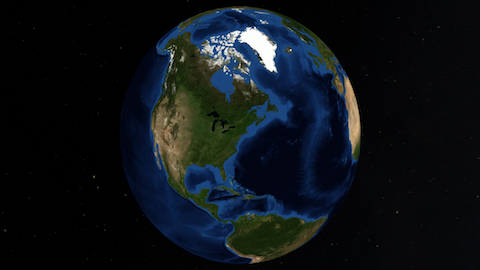
\includegraphics[width=\textwidth]{figures/results/os_view_earth.png}
        \caption{Earth}
    \end{subfigure}
    ~
    \begin{subfigure}[bt]{0.31\textwidth}
        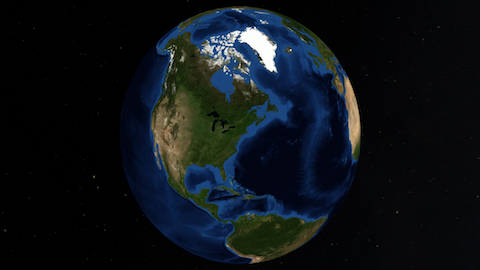
\includegraphics[width=\textwidth]{figures/results/os_view_earth.png}
        \caption{New York State}
    \end{subfigure}
    ~
    \begin{subfigure}[bt]{0.31\textwidth}
        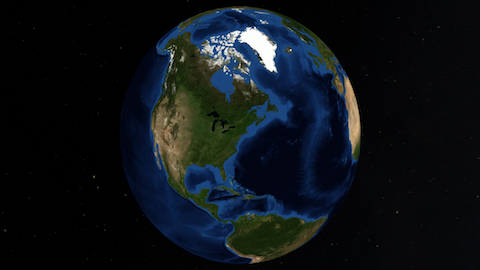
\includegraphics[width=\textwidth]{figures/results/os_view_earth.png}
        \caption{New York City}
    \end{subfigure}
    ~
    \begin{subfigure}[bt]{0.31\textwidth}
        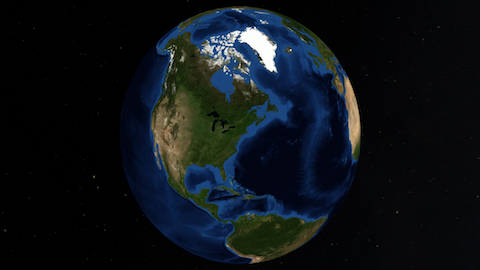
\includegraphics[width=\textwidth]{figures/results/os_view_earth.png}
        \caption{Manhattan}
    \end{subfigure}
    ~
    \begin{subfigure}[bt]{0.31\textwidth}
        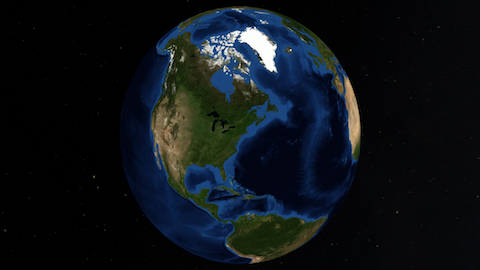
\includegraphics[width=\textwidth]{figures/results/os_view_earth.png}
        \caption{Central Park West}
    \end{subfigure}
    \caption{Top-down views of Earth at different zoom levels}
    \label{fig:topdown}
\end{figure}


\begin{table}
\centering
\caption[]{Top down settings}
  \label{table:settingstopdown}
  \begin{tabular}{| r | c c c c c |}
    \hline
      \textbf{Figure \ref{fig:topdown}}  & \textbf{a)} & \textbf{b)} & \textbf{c)} & \textbf{d)}  & \textbf{e)}  \\ \hline
      \textbf{Chunk Nodes}  & 10 & 54 & 66 & 102 & 106 \\ 
      \textbf{Leaf Chunk nodes} & 8 & 41 & 50 & 77 & 80 \\ 
      \textbf{Rendered Chunks} & 7 & 15 & 8 & 14 & 6 \\
      \textbf{Avg. FPS} & 48 & 42 & 42 & 40 & 41\\
    \hline
  \end{tabular}
\end{table}




\section{Benchmark: Horizontal view}

\subsection{Culling for Distance based LOD}

\subsection{Culling for Projected Area based LOD}

\section{Benchmark: Interactive Globe Browsing}

\section{Benchmark: Blending}

\section{Screenshots}
